%=========================================================
\chapter{Marco teórico}

\section{Ingeniería de software}

%El software se ha incrustado profundamente en casi todos los aspectos de nuestras vidas y, como consecuencia, el número de personas que tienen interés en las características y funciones que brinda una aplicación específica ha crecido en forma notable, por lo que debe hacerse un esfuerzo concertado para entender el problema antes de desarrollar una aplicación de software, por otro lado, los requerimientos de la tecnología de la información que demandan los individuos, negocios y gobiernos se hacen cada vez más complejos. En la actualidad, grandes equipos de personas crean programas de cómputo que antes eran elaborados por un solo individuo. El software sofisticado, que alguna vez se implementó en un ambiente de cómputo predecible y autocontenido, hoy en día se halla incrustado en el interior de todo, desde la electrónica de consumo hasta dispositivos médicos o sistemas de armamento. La complejidad de estos nuevos sistemas y productos basados en computadora demanda atención cuidadosa a las interacciones de todos los elementos del sistema.
%
%Hacer ingeniería con el software en todas sus formas y a través de todos sus dominios de aplicación, se ha convertido en una necesidad tangible . 
%
%El análisis es el proceso clave de la construcción de modernas aplicaciones de sistemas de información y la base para el diseño y desarrollo de la aplicación de software robusto y vigoroso. 

Una de las primeras definiciones de ingeniería de software fue dada por Fritz Bauer en el año de 1969, quien define que la ingeniería de software es “el establecimiento y uso de principios robustos, orientados a obtener software económico que sea fiable y que funcione de manera eficiente sobre máquinas reales” \hyperlink{b07}{[7]}, aunque esta definición omite algunos términos referentes a tiempos de entrega, procesos eficaces, y calidad de software, nos da un panorama de sus principios fundamentales y es también la base de la definición que la IEEE ha desarrollado de una manera más completa: 

"La ingeniería de software es: 1) La aplicación de un enfoque sistemático, disciplinado y cuantificable al desarrollo, operación y mantenimiento de software; es decir, la aplicación de la ingeniería al software. 
2) El estudio de enfoques según el punto 1"

La ingeniería de software está formada por un proceso, un conjunto de métodos (prácticas) y un arreglo de herramientas que permite a los profesionales elaborar software de cómputo de alta calidad. 

\begin{figure}[H]
	\begin{center}
		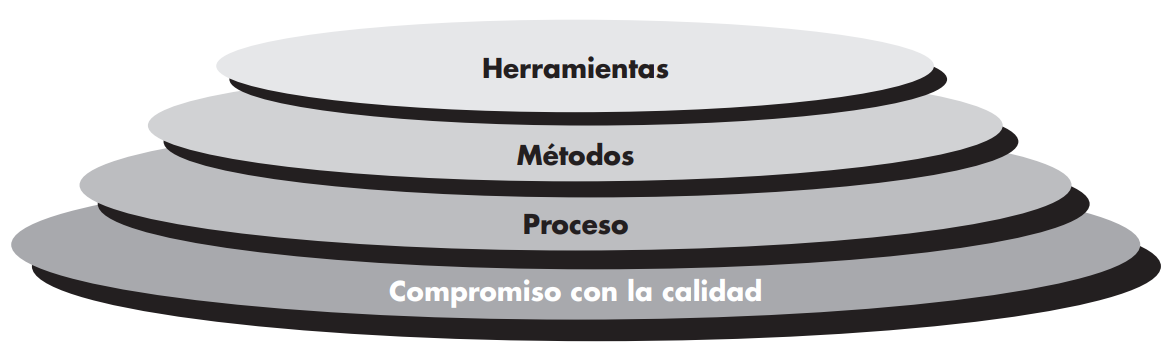
\includegraphics[width=.95\textwidth]{images/CapasIS}
		\caption{Capas de la ingeniería de software}
		\label{fig:capas_is}
	\end{center}
\end{figure}

La ingeniería de software es una tecnología con varias capas, como se muestra en la figura 3.1, existen 4 capas: herramientas, métodos, procesos y compromiso con la calidad. Cada una de ellas es importante, sin embargo, la capa de proceso es fundamental para el desarrollo de software, ya que es donde se define la estructura básica del producto hasta la culminación del mismo.

El proceso de software forma la base para el control de la administración de proyectos de software, y establece el contexto en el que se aplican métodos técnicos, se generan productos del trabajo (modelos, documentos, datos, reportes, formatos, etc.), se establecen puntos de referencia, se asegura la calidad y se administra el cambio de manera apropiada.

\subsection{Proceso de desarrollo de software}

Cuando se trabaja en la construcción de un producto o sistema, es importante ejecutar una serie de pasos predecibles, una estructura general para la ingeniería de software se define en cinco actividades elementales:

\begin{enumerate}
	\item Comunicación
	\item Planeación
	\item Modelado
	\item Construcción
	\item Despliegue
\end{enumerate}

Existen diferentes metodologías de desarrollo con modificaciones y adecuaciones al esquema general de construcción antes mencionado, algunas de ellas son las metodologías tradicionales y ágiles. Este proceso puede tener diferentes variaciones, sin embargo, sea cual sea la metodología aplicada, las etapas de Modelado (Análisis y Diseño) y Costrucción (Codificación y Pruebas) son las más críticas e importantes para un producto final exitoso.

Durante el desarrollo, se realizan tareas específicas para cada etapa, por ejemplo, para la etapa de modelado se elabora el documento de análisis (donde se describe el funcionamiento del sistema), así como el diseño (en donde se genrean los diagramas que describen el funcionamiento establecido en el análisis); en la fase de construcción se genera el código del software y en la etapa de pruebas se valida y verifica que el software cumpla con lo asentado en las fases precedentes.

\subsection{Modelado}

\subsubsection{Análisis}

El proceso de análisis dentro del desarrollo de software consiste en comprender y definir los requerimientos del sistema, evaluar las restricciones presenta, así como los insumos se requieren para su debida construcción.
Al ser la primera etapa dentro del proceso de desarrollo es las más crítica y sensible, ya que cualquier error que surja dentro de esta perjudicará las etapas consecuentes ocasionando retrasos en el proceso.
En esta etapa se construye el documento de análisis, en donde se describen todos los requerimientos que el cliente ha solicitado mediante diferentes componentes como lo son:

\begin{itemize}
	\item Reglas de negocio
	\item Mensajes
	\item Pantallas
	\item Casos de uso
	\item Entidades
\end{itemize}

 Este documento emplea un lenguaje técnico especializado ya que busca ser comprendido por los diseñadores y programadores para su correcta construcción.

\subsubsection{Caso de Uso}

Un caso de uso es una actividad que puede realizar un usuario dentro del software. Estas actividades sirven para describir el comportamiento del producto en distintas condiciones en las que el sistema responde a alguna de las peticiones realizadas por el usuario, es decir, describe el funcionamiento de
los componentes acorde a las acciones que los usuarios realizan dentro del software.
Un caso de uso está compuesto por distintos elementos, los cuales se describen a continuación: